\section{Реализация информационной системы}

\subsection{Описание работы системы}

При начальном запуске информационной системы, в терминале появляется меню, представленное на рисунке \ref{fig:login_menu.png}

\begin{figure}[h]
    \centering
    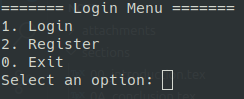
\includegraphics[width=0.6\textwidth]{login_menu.png}
    \caption{Меню входа в систему}
    \label{fig:login_menu.png}
\end{figure}

Блок схема данного алгоритма представлена на рисунке \ref{fig:diagram1}

\begin{figure}[h]
    \centering
    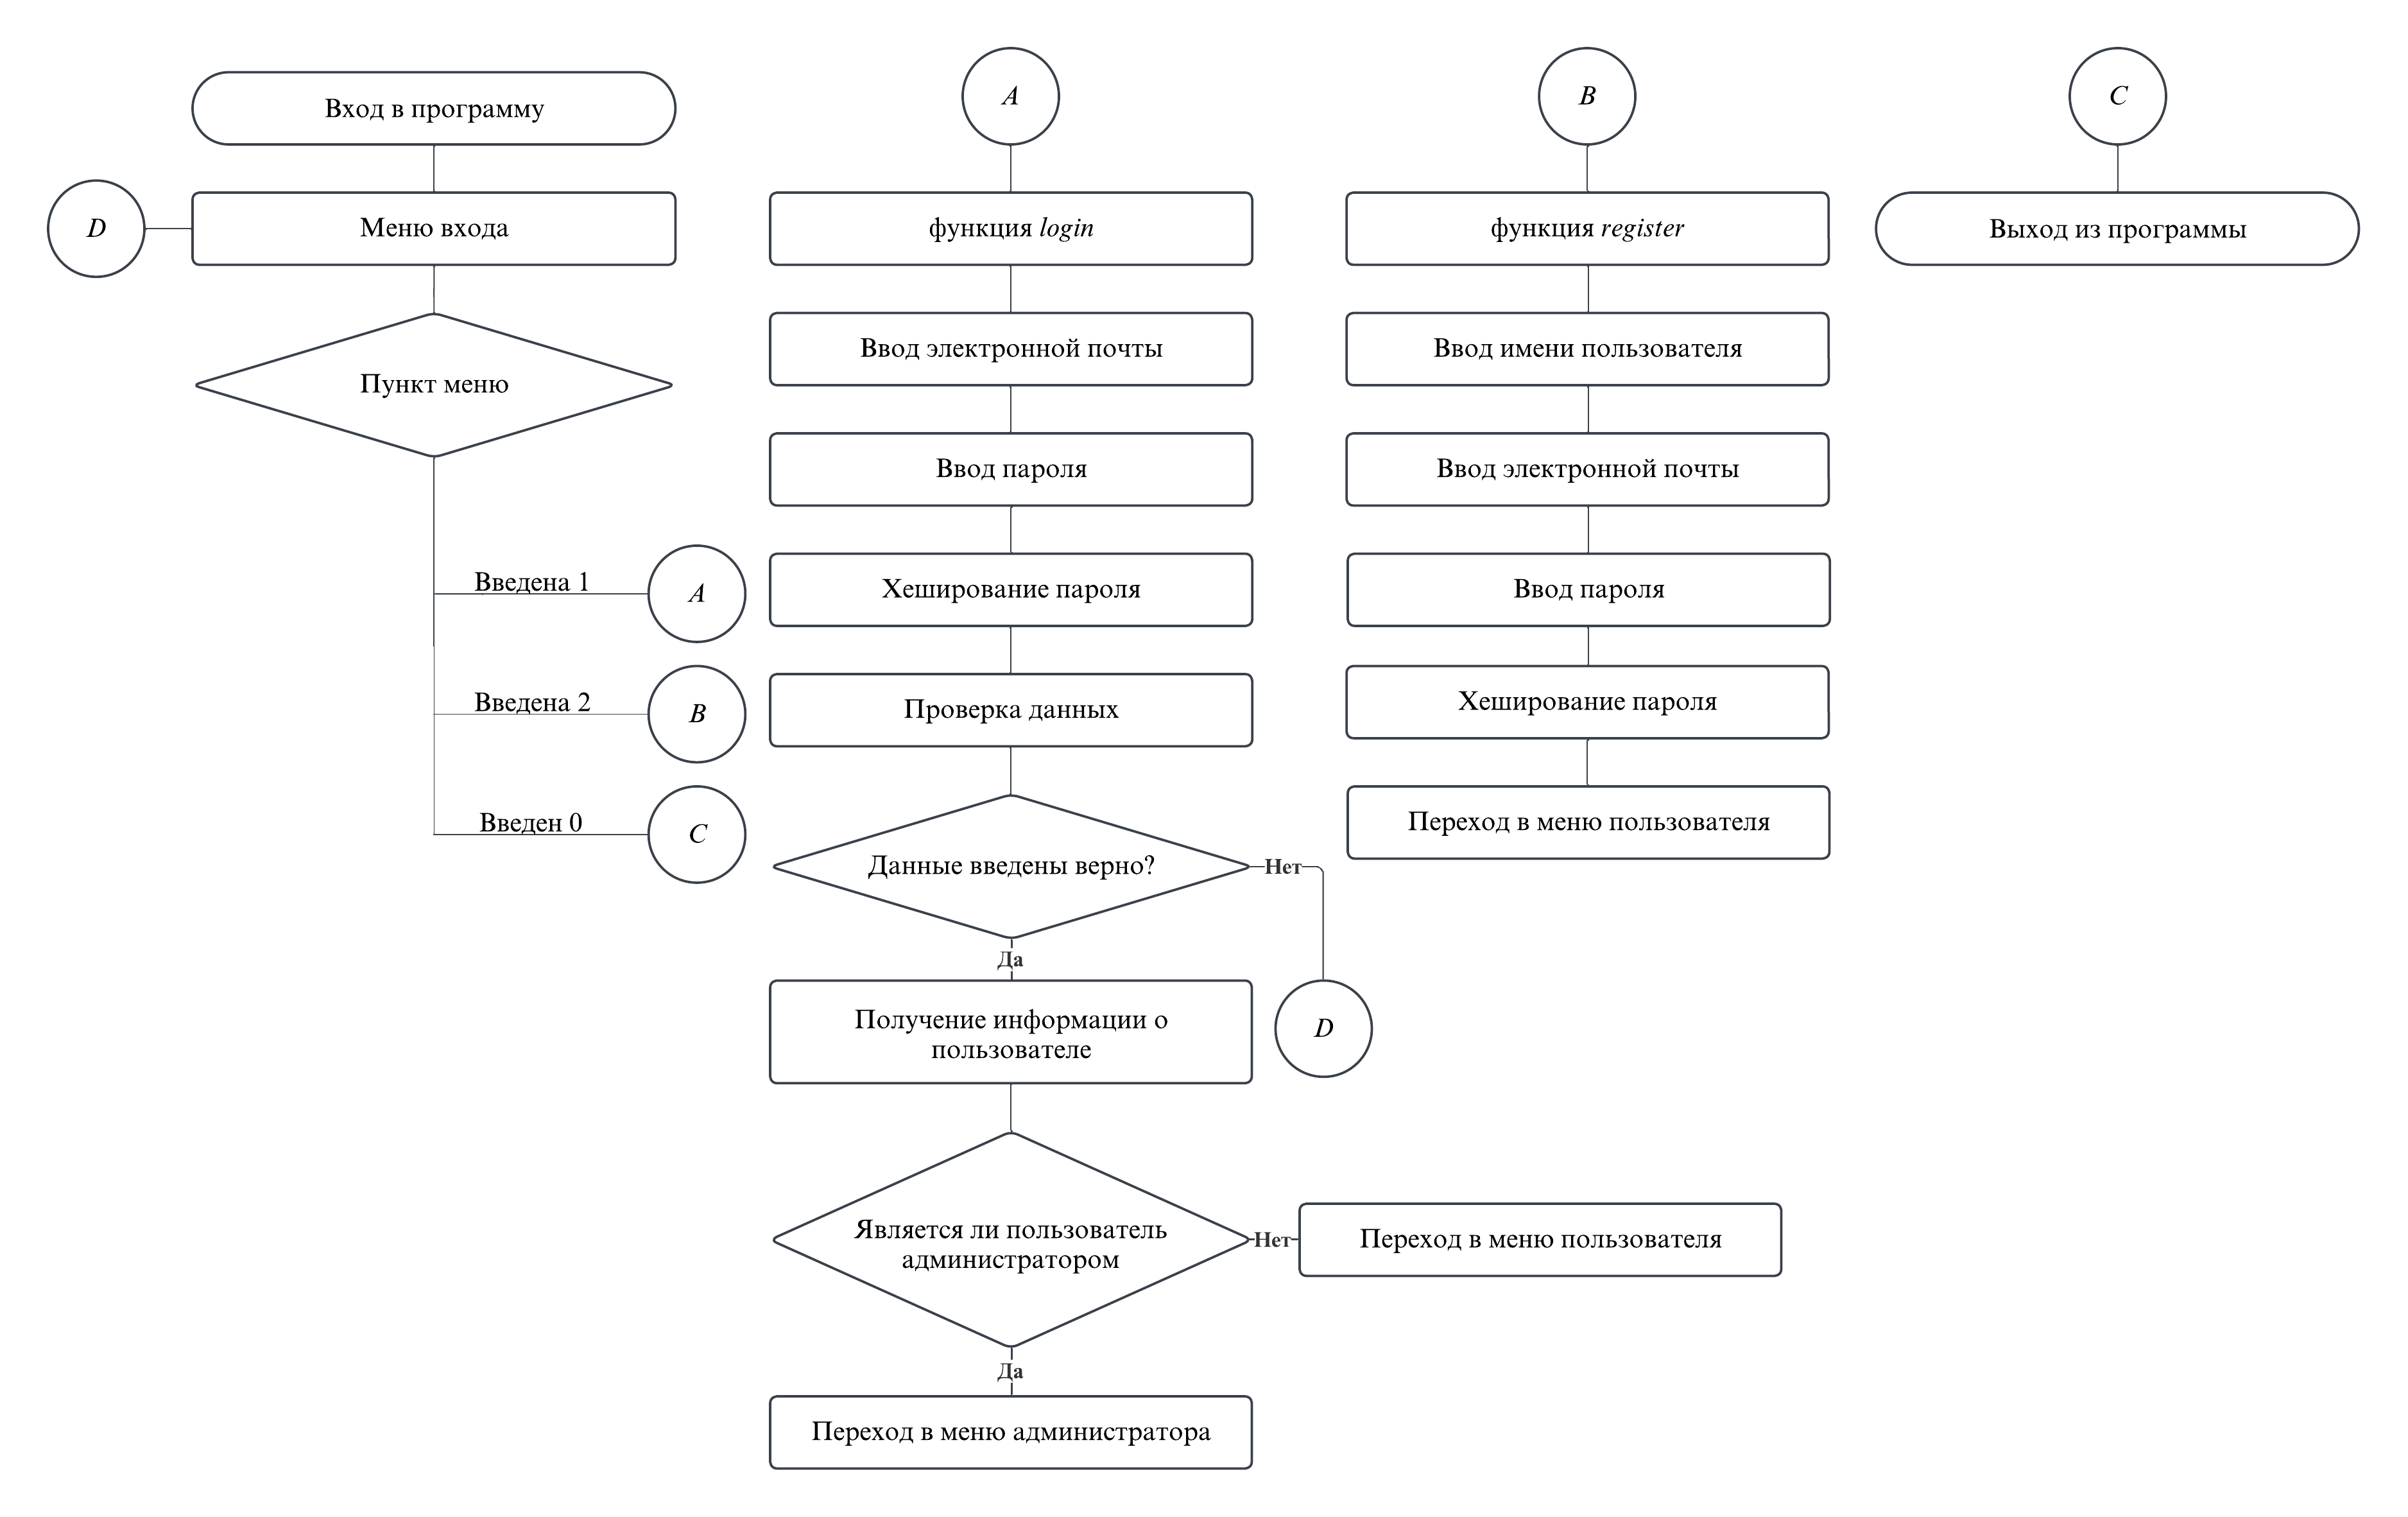
\includegraphics[width=1\textwidth]{diagram_login.png}
    \caption{Блок-схема алгоритма по входу}
    \label{fig:diagram1}
\end{figure}


Пользователю необходимо выбрать пункт меню. При вводе числа 0 система завершает свою работу (рисунок \ref{fig:login_exit.png})

\begin{figure}[h]
    \centering
    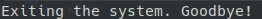
\includegraphics[width=0.6\textwidth]{login_exit.png}
    \caption{Демонстрация завершения сеанса}
    \label{fig:login_exit.png}
\end{figure}

Для того, чтобы у системы был красивый вид, после ввода каждой команды, терминал очищается.

Если пользователь введет число 2, система предложит зарегистрироваться. Работа функции для регистрации представлена на рисунке \ref{fig:registration_demonstration.png}.

\begin{figure}[h]
    \centering
    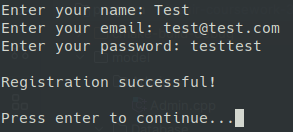
\includegraphics[width=0.6\textwidth]{registration_demonstration.png}
    \caption{Демонстрация регистрации}
    \label{fig:registration_demonstration.png}
\end{figure}

В системе предусмотрено то, что на одну электронную почту, можно создать только один аккаунт (рисунок \ref{fig:email_error.png})

\begin{figure}[h]
    \centering
    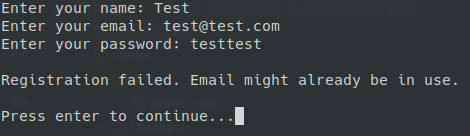
\includegraphics[width=0.4\textwidth]{email_error.png}
    \caption{Демонстрация ошибки о том, что почта уже привязана к другому аккаунту}
    \label{fig:email_error.png}
\end{figure}

Однако если регистрация пройдет успешно, то пользователь сразу же войдет в систему.

Также, если у пользователя есть аккаунт, он может войти в него, выбрав цифру 1. Для этого необходимо будет ввести \textit{email} и пароль, привязанный к аккаунту. 

В системе используется функция для хэширования паролей с использованием алгоритма \textit{SHA-256}, обеспечивающая высокий уровень безопасности. Хэширование представляет собой необратимый процесс преобразования исходного пароля в уникальную последовательность символов фиксированной длины. В данном случае для вычисления хэша применяется библиотека \textit{OpenSSL}. Поэтому пароли в системе хранятся безопасно и, при утечке данных, злоумышленники не смогут восстановить исходные значения паролей, так как процесс хэширования необратим. Даже если хэши будут получены, для нахождения исходного пароля потребуется выполнение вычислительно затратного перебора.

При регистрации, пользователь создается с правами доступа \text{User}. Рассмотрим систему со стороны пользователя. Меню выбора, для обычного пользователя представлено на рисунке \ref{fig:user_menu.png}

\begin{figure}[h]
    \centering
    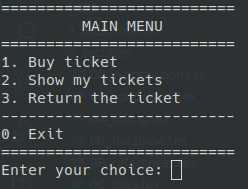
\includegraphics[width=0.4\textwidth]{user_menu.png}
    \caption{Меню выбора действия, для обычного пользователя}
    \label{fig:user_menu.png}
\end{figure}

По рисунку выше, понятно, что пользователь может проводить манипуляции только со своими билетами. Рассмотрим покупку билета (представлено на рисунке \ref{fig:create_ticket.png}).

\begin{figure}[h]
    \centering
    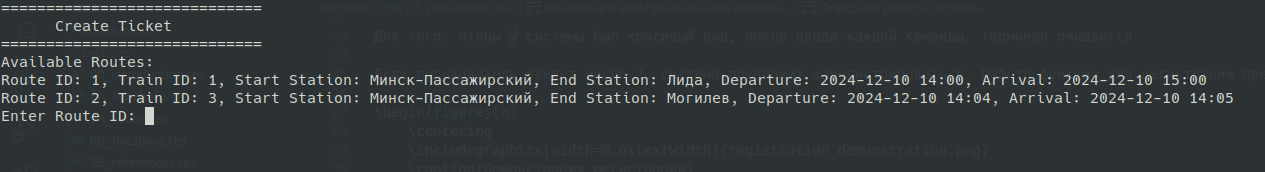
\includegraphics[width=1\textwidth]{create_ticket.png}
    \caption{Меню покупки билета}
    \label{fig:create_ticket.png}
\end{figure}

Затем, если выбрать корректный поезд, можно выбрать место посадки. В терминал выводятся абсолютно все свободные места (рисунок \ref{fig:choose_place.png}).

\begin{figure}[h]
    \centering
    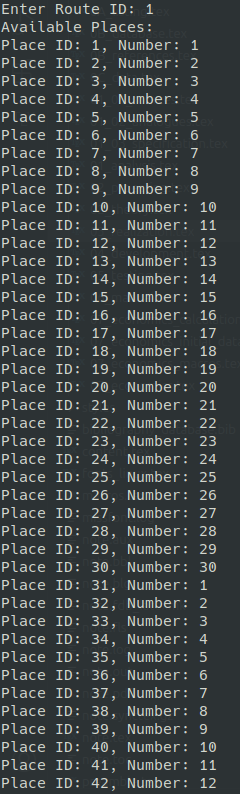
\includegraphics[width=0.25\textwidth]{choose_place.png}
    \caption{Фрагмент меню выбора места для посадки}
    \label{fig:choose_place.png}
\end{figure}

При этом, дата покупки билета фиксируется как текущая на момент оформления. Это позволяет системе автоматически сохранять временную метку без участия пользователя, обеспечивая точность и достоверность данных. Такое решение упрощает процесс покупки билетов и исключает вероятность ошибок при вводе даты вручную. Данный подход также облегчает последующий анализ данных, например, для статистики покупок или учета занятости мест. Дата сохраняется в таблице в формате \textit{YYYY-MM-DD HH:MM}.

Пользователь может в любое время просмотреть все свои билеты, получив полную информацию о каждом из них. В список включены такие данные, как уникальный идентификатор билета, название маршрута, номер места, дата и время отправления, а также место назначения. Это представлено наглядно в пользовательском интерфейсе (рисунок \ref{fig:read_tickets.png}).

\begin{figure}[h]
    \centering
    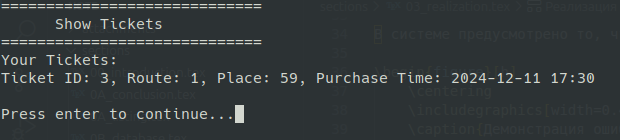
\includegraphics[width=0.8\textwidth]{ticket_read.png}
    \caption{Меню просмотра всех билетов пользователя}
    \label{fig:read_tickets.png}
\end{figure}

Кроме того, пользователь имеет возможность вернуть приобретённый билет. Возврат может быть осуществлён через интерфейс системы, где отображаются доступные для возврата билеты. Данный функционал позволяет пользователю гибко управлять своими поездками, например, изменяя планы или освобождая место для другого пассажира. При возврате билета данные обновляются в системе в реальном времени, что обеспечивает актуальность информации о доступных местах (рисунок \ref{fig:ticket_return.png}). 

\begin{figure}[h]
    \centering
    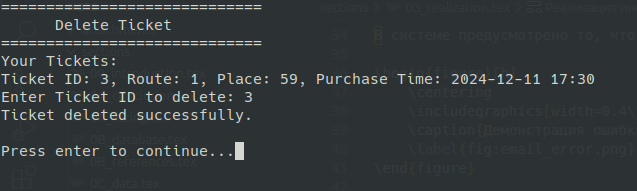
\includegraphics[width=0.8\textwidth]{ticket_return.png}
    \caption{Меню возврата билетов}
    \label{fig:ticket_return.png}
\end{figure}

Меню администратора в информационной системе вокзала предоставляет возможности для управления всеми ключевыми элементами инфраструктуры. Администратор может добавлять, редактировать и удалять поезда, указывая информацию о номере, маршруте, времени отправления и количестве вагонов. Для каждого поезда можно управлять вагонами, редактировать их параметры, включая типы и количество мест. Система позволяет управлять билетами, включая создание, изменение и удаление бронирований, а также назначать их на конкретные места в вагонах. Администратор может управлять станциями, путями и пользователями, обновлять их данные, а также следить за состоянием доступных мест и путевых маршрутов.

Рассмотрим некоторые ключевые функции, из тех, что перечислены выше. Каждая сущность в базе данных имеет полный набор \textit{CRUD}-запросов. 

\textit{CRUD} — это аббревиатура, обозначающая четыре основные операции, используемые для управления данными в базе данных: \textit{Create} (создание), \textit{Read} (чтение), \textit{Update} (обновление) и \textit{Delete} (удаление). Эти операции предоставляют полный набор инструментов для выполнения всех необходимых действий с сущностями в системе.

Система проверяет значение поля \textit{is_admin} в таблице \textit{entities} при входе пользователя, чтобы определить его уровень доступа. Если значение равно \textit{true}, пользователь получает права администратора и доступ к функциональности управления ключевыми объектами системы, такими как поезда, вагоны, места, билеты, пути, станции и пользователи. В противном случае, пользователь рассматривается как обычный клиент с доступом только к покупке и просмотру билетов. Добавление нового администратора возможно только вручную через прямое изменение записей в базе данных, что обеспечивает дополнительный уровень безопасности и контроля.

Меню администратора представлено на рисунке \ref{fig:admin_menu}.

\begin{figure}[h]
    \centering
    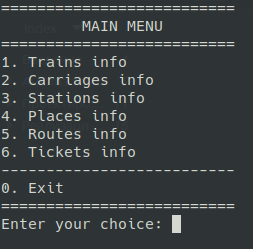
\includegraphics[width=0.5\textwidth]{admin_menu.png}
    \caption{Меню администратора}
    \label{fig:admin_menu}
\end{figure}

В нем, так же как и в меню обычного пользователя, можно выбирать различные пункты меню. Рассмотрим ключевые функции некоторых пунктов меню.

Меню поездов представлено на рисунке \ref{fig:trains_menu}. Информационная система предоставляет функции для добавления, удаления и просмотра поездов.

\begin{figure}[h]
    \centering
    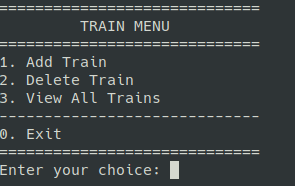
\includegraphics[width=0.7\textwidth]{trains_menu.png}
    \caption{Меню поездов}
    \label{fig:trains_menu}
\end{figure}

Рассмотрим добавление поезда. Для добавления поезда необходимо ввести его номер, а также тип поезда (рисунок \ref{fig:create_train}).

\begin{figure}[h]
    \centering
    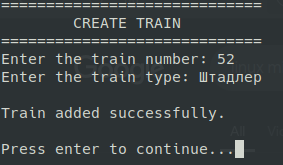
\includegraphics[width=0.8\textwidth]{create_train.png}
    \caption{Функционал по добавлению поезда в базу данных}
    \label{fig:create_train}
\end{figure}

Также, рассмотрим удаление поезда по его идентификатору. При попытке удаления поезда, система выводит список всех доступных поездов. Удалим поезд номер 7, а затем попробуем прочитать список всех доступных поездов (рисунок \ref{fig:delete_trains} и рисунок \ref{fig:read_trains})


При удалении поезда по его идентификатору система выполняет несколько последовательных шагов для обеспечения корректности операций.

Во-первых, при запросе на удаление система выводит пользователю актуальный список всех доступных поездов, чтобы он мог визуально подтвердить данные о поезде, который требуется удалить. Это особенно важно для предотвращения ошибок, связанных с удалением неправильного объекта.

Например, если пользователь выберет удаление поезда, идентификатор которого равен 7, система проверит его наличие в базе данных. Если поезд с таким идентификатором существует, он будет удален. При этом система также автоматически удаляет связанные с этим поездом данные, такие как вагоны, места и билеты, чтобы избежать несоответствий в базе данных.

После выполнения операции удаления пользователь может запросить обновленный список доступных поездов. Система вновь выполнит запрос к базе данных и отобразит актуальную информацию, из которой теперь будет исключен поезд с идентификатором 7. Это наглядно продемонстрировано на рисунках \ref{fig:delete_trains} и \ref{fig:read_trains}, где показано состояние данных до и после удаления поезда.

\begin{figure}[h]
    \centering
    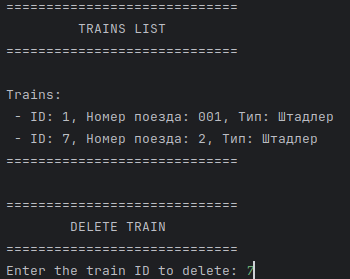
\includegraphics[width=0.7\textwidth]{delete_trains.png}
    \caption{Удаление поезда с идентификатором 7}
    \label{fig:delete_trains}
\end{figure}

\begin{figure}[h]
    \centering
    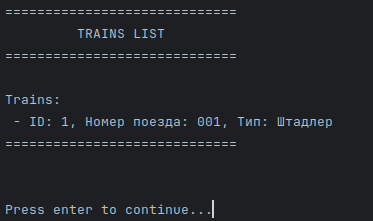
\includegraphics[width=0.7\textwidth]{read_trains.png}
    \caption{Список всех поездов после удаления поезда с идентификатором 7}
    \label{fig:read_trains}
\end{figure}

На рисунке \ref{fig:read_trains} видно, что поезда с идентификатором 7 больше нету в базе данных.

Теперь рассмотрим операции над вагонами. По рисунку \ref{fig:struct_db} видно, что у таблицы \textit{carriage} есть зависимость от \textit{trains}. Также, в каждом вагоне есть места. Рассмотрим создание нового вагона (рисунок \ref{fig:create_carriage}). При создании вагона, система выполняет несколько последовательных операций: создание записи в таблице \textit{carriage}, а также наполнение его местами. Это сделано для того, чтобы упростить задачу по созданию мест. В каждом вагоне может быть от 30 мест. Программа создает 30 мест. Чуть позже, с помощью меню по управлению местами, администратор может корректировать их количество.

От администратора система требует идентификатор существующего поезда. При этом, система показывает список всех поездов, а если их нет, то система оповестит об этом администратора. Затем система требует номер вагона и его тип.

\begin{figure}[h]
    \centering
    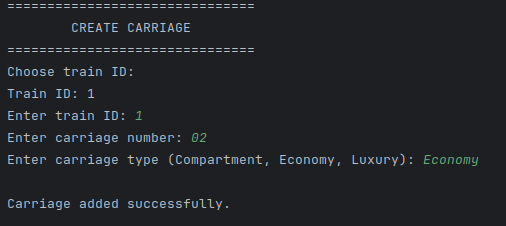
\includegraphics[width=0.7\textwidth]{create_car.png}
    \caption{Функционал по созданию вагона}
    \label{fig:create_carriage}
\end{figure}

Не будем рассматривать как удаляются вагоны. Все выглядит так же, как и с поездами. Аналогично с просмотром всех доступных вагонов.

Рассмотрим меню по управлению путями (рисунок \ref{fig:routes_menu}).

\begin{figure}[H]
    \centering
    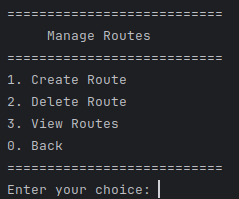
\includegraphics[width=0.5\textwidth]{routes_menu.png}
    \caption{Меню управления поездками}
    \label{fig:routes_menu}
\end{figure}

При разработке информационной системы для вокзала функции удаления и просмотра различных сущностей реализуются по аналогичному принципу, что и для других элементов системы, таких как поезда, вагоны, станции и билеты. Эти действия требуют простого выполнения запросов к базе данных, что позволяет быстро и эффективно обрабатывать соответствующие запросы. В связи с этим, более детальное рассмотрение их реализации в данном разделе нецелесообразно. Вместо этого акцент далее сделан на рассмотрении процесса создания сущностей, поскольку это сложная и важная часть функционала системы.

Поездка в данной информационной системе является составной сущностью, включающей поезд, вагоны и две станции — станцию отправления и станцию прибытия. При создании новой поездки требуется указать существующий поезд из базы данных, что обеспечивает связь поездки с реальными данными о составе. Также указываются станции отправления и прибытия, которые должны быть предварительно внесены в базу данных. Для обеспечения корректности планирования необходимо задать время отправления и прибытия, что позволяет учитывать расписание движения поездов и гарантировать точность работы системы (рисунок \ref{fig:create_route}).

\begin{figure}[H]
    \centering
    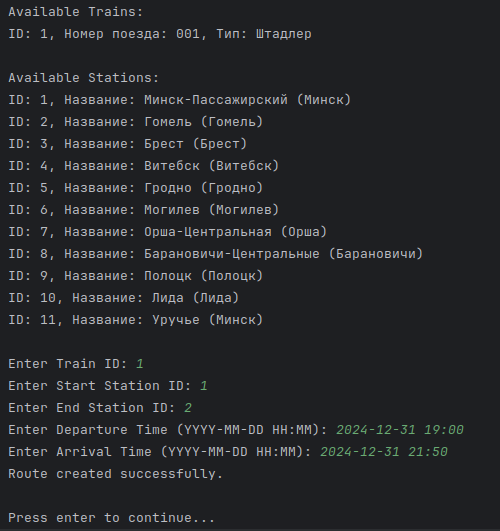
\includegraphics[width=0.5\textwidth]{create_route.png}
    \caption{Функционал по созданию поездки}
    \label{fig:create_route}
\end{figure}

Рассмотрим удаление поездки. Удаление поездки представлено на рисунке \ref{fig:delete_route}

\begin{figure}[H]
    \centering
    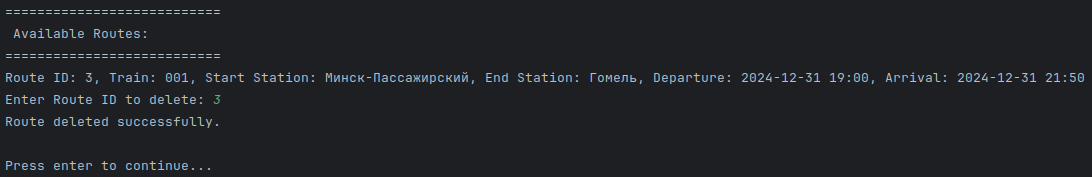
\includegraphics[width=1\textwidth]{delete_route.png}
    \caption{Функционал по удалению поездки}
    \label{fig:delete_route}
\end{figure}

От администратора система требует идентификатор существующей поездки. При этом, система показывает список всех поездок, а если их нет, то система оповестит об этом администратора(рисунок \ref{fig:empty_routes}). 

\begin{figure}[H]
    \centering
    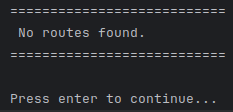
\includegraphics[width=0.7\textwidth]{empty_routes.png}
    \caption{Оповещение системы о том, что поездки отсутствуют}
    \label{fig:empty_routes}
\end{figure}

Рассмотрим меню билетов(рисунок \ref{fig:tma})

\begin{figure}[H]
    \centering
    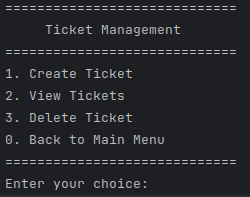
\includegraphics[width=0.6\textwidth]{tma.png}
    \caption{Меню билетов}
    \label{fig:tma}
\end{figure}

Расссмотрим функцию создания билета(рис \ref{fig:ct1} и \ref{fig:ct2}).

\begin{figure}[H]
    \centering
    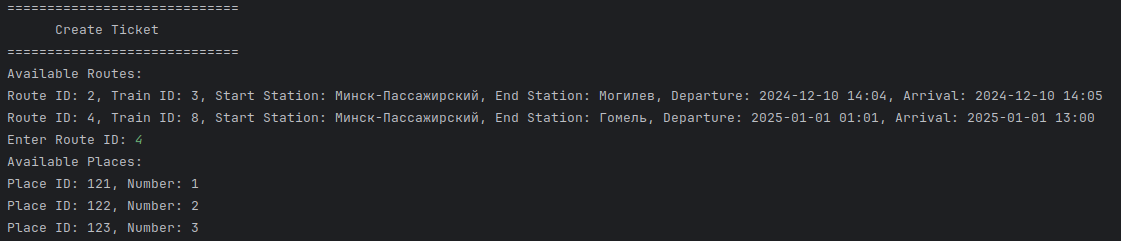
\includegraphics[width=0.7\textwidth]{ct1.png}
    \caption{Функционал по созданию билета ч.1}
    \label{fig:ct1}
\end{figure}

\begin{figure}[H]
    \centering
    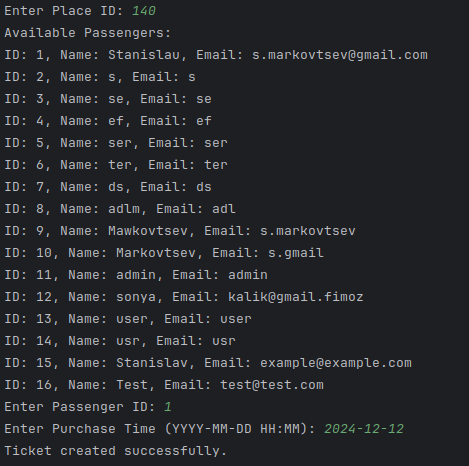
\includegraphics[width=0.7\textwidth]{ct2.png}
    \caption{Функционал по созданию билета ч.2}
    \label{fig:ct2}
\end{figure}

В отличии от функции покупки билета в меню пользователя(\ref{fig:create_ticket.png}), в создании билета в меню администратора пассажир, а так же дата покупки задаются вручную.

Также в системе есть вспомогательные функции:

\begin{itemize}
    \item функция \textit{handleInvalidInput()} -- функция вызывается после каждого пользовательского ввода. Она нужна для того, чтобы после некорректного ввода, программа не завершала свою работу.
    \item функция \textit{clearScreen()} -- функция вызывается перед каждым пользовательским вводом. Она нужна для того, чтобы интерфейс создавал впечатление обновления экрана.
    \item функция \textit{pressToContinue()} -- функция вызывается после завершения какого то блока программы, например перед \textit{break} или \textit{return}.
    \item функция \textit{hashPassword()} -- функция используется для безопасного хранения паролей в базе данных.
    \item функция \textit{getCurrentTime} -- функция используется для получения текущего времени. Например, когда пользователь оформляет билет.
\end{itemize}
